\chapter{Multiplicitetsföljder}

I detta kapitel ska vi studera singulariteter hos singulära algebraiska kurvor och presentera ett sätt hur dessa kan klassificeras. Precis som i kapitel \ref{Curves} kan vi anta att kurvorna går igenom origo, samt att singulariteten vi ska studera ligger i origo. Men först ska vi titta på hur vi kan förenkla en singularitet med hjälp av att \emph{blåsa upp dem} i en högre dimension, i ett försök att göra kurvan mjukare.

\section{Uppblåsningar}

Låt oss först titta på den plana algebraiska kurvan $C(t)=(t^2,t^3+t^7)$. I exempel \ref{ImplicitNotationEx3} ser vi att denna kurva ges implicit av ekvationen
\[y^2-x^3-2x^5-x^7 = 0\]
Vi ser också att den har en singularitet i origo. Kurvan ser ut som följer runt denna singularitet:

\begin{center}
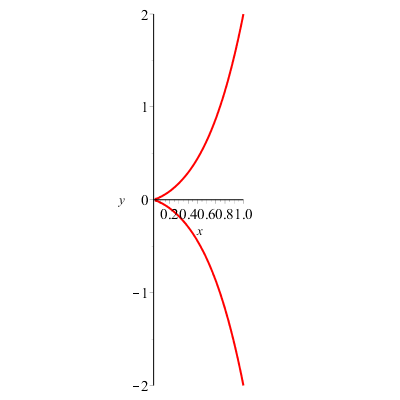
\includegraphics[scale=0.35]{Export/blowupex1_1.png}
\end{center}

Ett sätt att mjuka upp kurvan, utan att förändra den, eller att den förlorar någon av sin inneboende information, är att se den som en projektion av en kurva från en högre dimension. Denna senare kurva kan mycket väl vara mjuk. I det fallet då den algebraiska kurvan är given i parametriserad form, som $C(t)=\left(x(t),y(t)\right)$, är det dessutom enkelt att skapa en mjukare variant av kurvan i tre dimensioner. Detta görs enklast genom att införa $z(t)=t$ som en tredje dimension: $C^*(t)=\left(x(t),y(t),z(t)\right)$. I vårt exempel ovan skulle detta ge $C^*(t)=(t^2,t^3+t^7,t)$, vilken visas i nedanstående graf. I grafen finns även tre projektioner utritade ($P_x(t)=(x_p,y(t),z(t))$, $P_y(t)=(x(t),y_p,z(t))$ och $P_z(t)=(x(t),y(t),z_p)$), den ena ($P_z(t)$) liknar vår originalkurva.

\begin{center}
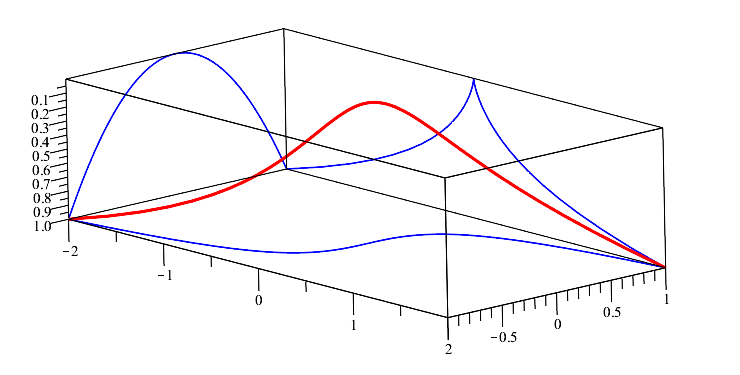
\includegraphics[scale=0.5]{Export/blowupex1_2.png}
\end{center}

Men hur gör vi med en algebraisk kurva som ges implicit av en polynomekvation $F(x,y)=0$? Att ta fram en parametrisering för en sådan kurva är inte helt enkelt i det generella fallet. Istället kan vi införa en tredje dimension till kurvan genom att utanför singulariteten introducera $z=y/x, x \neq 0$. Ritar vi upp den resulterande kurvan för vårt exempel, tillsammans med de tre projektionerna, får vi:

\begin{center}
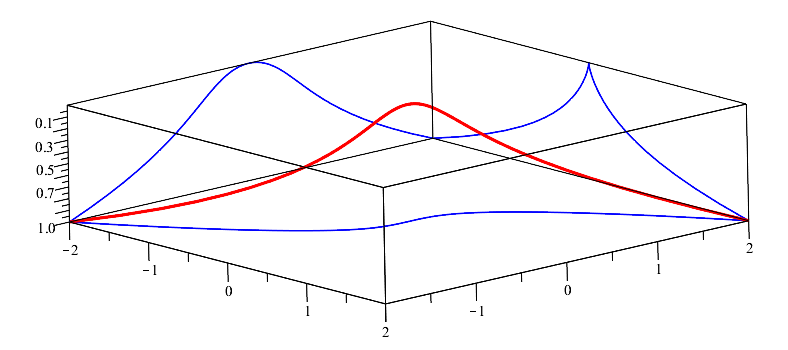
\includegraphics[scale=0.5]{Export/blowupex1_3.png}
\end{center}

Eftersom vår ursprungliga kurva uppfyller $F(x,y)=0$ och den nya kurvan även uppfyller $z=y/x$, och därför $y=z\cdot x$, måste den nya kurvan således även uppfylla
\[F(x,z\cdot x)=0\]

I vårt exempel ger detta således:

\[
\begin{array}{c}
(z\cdot x)^2-x^3-2x^5-x^7 = x^2 \cdot \left(z^2-x-2x^3-x^5\right) = 0 \Longrightarrow\\[5pt]
\Longrightarrow z^2-x-2x^3-x^5=0\\
\end{array}
\]

Således får vi en ny kurva $C^*$, implicit givet av polynomekvationen $F^*(x,z)=z^2-x-2x^3-x^5=0$ vilken är \emph{enklare} än den ursprungliga polynomekvationen $F(x,y)=0$. Denna nya kurva $C^*$ motsvarar precis projektionen $P_y$ av vår tredimensionella kurva på XZ-planet:

\begin{center}
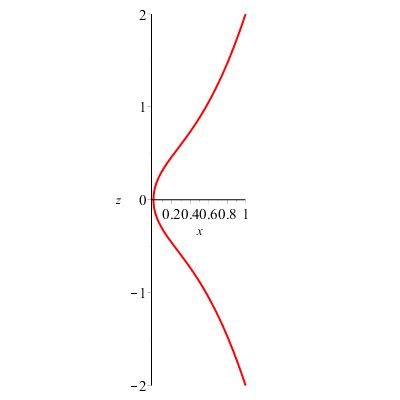
\includegraphics[scale=0.5]{Export/blowupex1_4.png}
\end{center}

Vi ser att ovanstående operation genererar en ny kurva som är enklare än den första, samt att denna nya kurva är relaterad till den första kurvan genom att båda är projektioner av samma kurva från en högre dimension. Detta leder oss till följande generalisering för att se om detta resultat är mer generellt:

\begin{Definition}
\label{BlowUp}
En \textbf{uppblåsning} av en algebraisk plan singulär kurva $C$ som går genom origo, givet implicit genom polynomekvationen $F(x,y)=0$, är den algebraiska plana kurva $C^*$ som ges implicit av $F^*(x,y) = F(x,x\cdot y)/x^m=0$, där $m$ är \textbf{multipliciteten} av nollstället $x=0$ i $F(x,x\cdot y)$, dvs. det största heltal $m$ sådant att $x^m$ delar alla termer i $F(x,x\cdot y)$.
\end{Definition}

\begin{Theorem}
\label{MultiplicityPositive}
För multipliciteten gäller att $m > 0$ om $F(x,y)$ går igenom origo.
\end{Theorem}

\begin{proof}
Att $m>0$ följer mer eller mindre direkt av definitionen: $F(x,y)$ är ett polynom. Kurvan går genom origo, så $F(0,0)=0$, vilket innebär att $F(x,y)$ saknar konstant term. Således innehåller alla termer i $F(x,y)$ minst ett $x$ eller ett $y$. I båda fallen ser vi att $x$ delar både $x$ själv och $x\cdot y$. Således delar $x$ hela $F(x,x\cdot y)$, och således är $m$ minst 1.
\end{proof}

I bilaga \ref{BlowUpXY} finns beskrivet en algoritm som beräknar uppblåsningen $F^*(x,y)$ av en kurva, givet dess implicita form $F(x,y)=0$, samt motsvarande multiplicitet $m$.

\section{Multiplicitetsföljder}

Vi har nu sett att vi kan skapa en uppblåsning $F^*(x,y)$ av en funktion $F(x,y)$, samt en motsvarande multiplicitet $m$. Nu ska vi undersöka vad som händer om vi upprepar denna process iterativt, och även se hur långt vi kan upprepa den. Låt oss kalla uppblåsningsoperatorn definierad ovan för $B$ (för ``Blow-Up''), där $F(x,y)$ blåses upp till $F^*(x,y)$ och $m$ är den implicit genererade multipliciteten i operationen:

\[F \overset{B}{\underset{m}{\longrightarrow}} F^*\]

Anta att vi har en serie uppblåsningar:

\[
F(x,y) \overset{B}{\underset{m_1}{\longrightarrow}} F_1(x,y) \overset{B}{\underset{m_2}{\longrightarrow}} \ldots \overset{B}{\underset{m_n}{\longrightarrow}} F_n(x,y) \overset{B}{\underset{m_{n+1}}{\longrightarrow}} \ldots
\]

Denna serie kan bara fortgå så länge $F_i(x,y)$ är singulär i origo. Hur länge är det? Låt oss betrakta $F(x,y)=y^2-xy$:

\[
(y^2-xy) \overset{B}{\underset{2}{\longrightarrow}} (y^2-y) \overset{B}{\underset{1}{\longrightarrow}} (xy^2-y) \overset{B}{\underset{1}{\longrightarrow}} (x^2y^2-y) \overset{B}{\underset{1}{\longrightarrow}} (x^3y^2-y) \overset{B}{\underset{1}{\longrightarrow}} \ldots
\]

Multiplicitetsföljden blir $2,1,1,1,1,\ldots$, i all oändlighet. Anledningen till detta är att alla termer innehåller $y$ som alltid genererar en faktor $x$ för varje uppblåsning.

\begin{Theorem}
\label{FiniteMultiplicitySequence}
Om $F(x,y)\in \mathbb{C}[x,y]$ är singulär i origo och är summan av ett polynom $G(x,y)=y\cdot H(x,y)$, vilket har minst ett $y$ i varje term, och ett polynom $p(x) \neq 0$ som bara har termer bestående av potenser av $x$, så är multiplicitetsföljden av $F(x,y)$ en ändlig serie av icke strikt avtagande heltal.
\end{Theorem}

\begin{proof}
Låt $n=\mathbf{o}(p)$. Vi har här att $F(x,y)=G(x,y)+x^nq(x)$ för något polynom $q(x)$ sådant att $q(0)\neq 0$. Alla termer i $G(x,y)$ har en multipel av $y$ i sig. ($G(x,y)$ kan inte ha en konstant term, då $G(0,0)=0$.) Applicerar vi uppblåsningsoperatorn successivt får vi:

\[
\begin{array}{c}
G(x,y)+x^nq(x) \overset{B}{\underset{m_1}{\longrightarrow}} G_1(x,y)+x^{n-m_1}q(x) \overset{B}{\underset{m_2}{\longrightarrow}} \ldots \overset{B}{\underset{m_i}{\longrightarrow}} \\[15pt]
\overset{B}{\underset{m_i}{\longrightarrow}} G_i(x,y)+x^{n-\sum_{j=1}^{i}m_j}q(x) \overset{B}{\underset{m_{i+1}}{\longrightarrow}} \ldots \\
\end{array}
\]

För sekvensen av polynom $G_i(x,y)$ gäller följande: De har fortfarande samma antal termer som $G(x,y)$. Operatorn påverkar inte potenserna av $y$ i sig, bara faktorer innehållande potenser av $x$. Men eftersom alla termer innehåller minst ett $y$, ändras inte antalet termer. Varje term kommer dessutom alltid kunna bidra med minst graden av $y$ till multipliciteten plus eventuella potenser av $x$ som är kvar. Detta gör också att $G_i(x,y)$ alltid kommer sakna konstantterm och därför också gå igenom origo. Så länge $\sum_{j=1}^{i}m_j<n$ kommer således hela $G_i(x,y)+x^{n-\sum_{j=1}^{i}m_j}q(x)$ också gå genom origo. Men sats \ref{MultiplicityPositive} säger att då detta gäller är multipliciteterna alltid positiva, vilket leder till att sekvensen måste få ett stopp efter $N$ steg för något $N$ sådant att $\sum_{j=1}^{N}m_j=n$. Detta leder till att den sista uppblåsningen blir $G_N(x,y)+q(x)$, vilket inte går genom origo, och uppblåsningssekvensen avbryts.

Att $m_i \geq m_{i+1}, \forall i$ ser man på följande sätt: Först ordnar vi om $F(x,y)$ och tittar på det som om det vore ett polynom i $y$:
\[F(x,y) = \sum_{i\in I} p_i(x)y^i = \sum_{i\in I} x^{n_i}q_i(x)y^i\]
för någon mängd $I$ med exponenter till $y$, och där $n_i=\mathbf{o}(p_i)$ och $q_i(0)\neq 0$, dvs. $x \nmid q_i(x)$. Vi ser här att $p(x)=p_0(x)$ och $q(x)=q_0(x)$ enligt ovanstående antagande. Vi applicerar sedan uppblåsnings\-operatorn:

\[F(x,y) \overset{B}{\underset{m_1}{\longrightarrow}} \frac{F(x,x\cdot y)}{x^{m_1}}=\sum_{i\in I} x^{n_i+i-m_1}q_i(x)y^i\]

Vi ser här att $m_1$ bara beror på talföljden $\left\{n_i+i\right\}_{i\in I}$. Vi ser också att
\[m_1=\min(\left\{n_i+i\right\}_{i\in I})\]
$m_1$ kan inte vara mindre, för då skulle vi kunna dela resultatet med ett $x$ till, i strid med vår definition av uppblåsningsoperatorn. Den kan inte vara större heller, då $x^{n_i+i-m_1}$ då skulle bli negativt för något $i$, också det i strid med vår definition av uppblåsningsoperatorn. Vi applicerar operatorn en gång till (om det är tillåtet, annars är vi klara):

\[\ldots \overset{B}{\underset{m_2}{\longrightarrow}} \sum_{i\in I} x^{n_i+(i-m_1)+(i-m_2)}q_i(x)y^i\]

Vi vet att $\exists i_1:n_{i_1}+i_1-m_1=0$. (Hade alla $n_i+i-m_1$ varit positiva, hade vi kunnat dela med fler $x$ i första uppblåsningsoperatorn.) Men det betyder att $m_2\leq i_1$, annars skulle $x$-exponenten bli negativ för just den termen. Men $i_1=m_1-n_{i_1}\leq m_1$. Således är $m_2\leq m_1$.

Vi antar nu att $m_1\geq m_2 \geq \ldots \geq m_k, k \geq 2$. Vi applicerar uppblåsnings\-operatorn ännu en gång och får:

\[\ldots \overset{B}{\underset{m_{k+1}}{\longrightarrow}} \sum_{i\in I} x^{n_i+\sum_{j=1}^{k} (i-m_j) + (i-m_{k+1})}q_i(x)y^i\]

Om nu $m_{k+1}>m_k$ ser vi att vi hade kunnat subtrahera ytterligare från exponenten i tidigare skede (i exponentens $(i-m_k)$-term) genom att göra $m_k$ större, vilket motsäger det faktum att $m_k$ är det största heltal som jämnt delar alla termer i föregående uppblåsningsoperation. Alltså måste $m_{k+1}\leq m_k$, och således, genom induktion, är hela multiplicitetsföljden en ändlig icke strikt avtagande följd
\[m_1 \geq m_2 \geq \ldots \geq m_N\]
\end{proof}

\begin{Corollary}
\label{OrderP}
Givet $F(x,y)=y\cdot H(x,y)+p(x)$ från sats \ref{FiniteMultiplicitySequence}, och dess multiplicitetsföljd $\left\{m_i\right\}$, gäller att $\mathbf{o}(p)=\sum m_i$.
\end{Corollary}

\begin{proof}
Detta fås direkt ur första delen av beviset av sats \ref{FiniteMultiplicitySequence}.
\end{proof}

Om vi går tillbaka till vår oändliga multiplicitetsföljd vi fick genom att successivt blåsa upp $F(x,y)=y^2-xy$ kan vi notera att $y^2-xy=y(y-x)$ inte är irreducibel, och att nollmängden till ekvationen $F(x,y)=y^2-xy=y(y-x)=0$ består av två linjer: $y=0$ och $y=x$. Det kan vara värt att notera att kravet att $F(x,y)$ ska vara \emph{irreducibel} är ett strängare krav än det i sats \ref{FiniteMultiplicitySequence}, och att det därför också garanterar att multiplicitetsföljden är ändlig och icke strikt avtagande.

\begin{Corollary}
Om $F(x,y)\in \mathbb{C}[x,y]$ är ett irreducibelt polynom som är singulärt i origo, så är multiplicitetsföljden av $F(x,y)$ en ändlig serie av icke strikt avtagande heltal.
\end{Corollary}

\begin{proof}
Vi måste visa att $F(x,y)$ är summan av ett polynom $G(x,y)=y\cdot H(x,y)$, vilket har minst ett $y$ i varje term, och ett polynom $p(x) \neq 0$ som bara har termer bestående av potenser av $x$. Men detta följer av det faktum att $F(x,y)$ måste ha en term av typen $x^n$ och en term av typen $y^m$ för några $m$ och $n$. Om den skulle sakna termer av typen $x^n$ skulle alla termer ha minst ett $y$, och man skulle således kunna byta ut en faktor $y$ ur $F(x,y)$, vilket motsäger att det är irreducibelt. På samma sätt ser vi att det $F(x,y)$ måste ha minst en term $y^m$, annars skulle man kunna bryta ut en faktor $x$ ur $F(x,y)$. Således kan vi samla alla termer i $F(x,y)$ som har $y$ i sina termer i polynomet $G(x,y)$, och resterande termer som bara innehåller $x$ i $p(x)$. Båda dessa två kommer innehålla termer, eftersom $F(x,y)$ är irreducibelt. Således är multiplicitetsföljden en ändlig serie av icke strikt avtagande heltal, enligt sats \ref{FiniteMultiplicitySequence}.
\end{proof}

I bilaga \ref{MultiplicitySequenceXY} finns beskrivet en algoritm som beräknar multiplicitetsföljden för ett polynom $F(x,y)$, givet att det kan skrivas på formen given i sats \ref{FiniteMultiplicitySequence}. Där finns också flera exempel som visar olika multiplicitetsföljder för olika polynom.

\section{Funktionsfamiljer}

Nu när vi har en metod att skapa en multiplicitetsföljd $\left\{m_i\right\}$ från ett polynom $F(x,y)$, kan vi ställa oss den omvända frågan: Givet en multiplicitetsföljd $\left\{m_i\right\}$, hur ser funktionerna $F(x,y)$ ut som har motsvarande multiplicitetsföljd?

I bilaga \ref{FindFunctionXYFromMultiplicitySequence} presenteras en algoritm som beräknar en familj av funktioner som alla genererar en given multiplicitetsföljd. Funktionen som implementerar algoritmen returnerar också den enklaste lösningen från denna familj. Algoritmen är relativt enkel. Huvuddragen är som följer:

\begin{enumerate}
\item Först skapas en ansats på lösning. Om $\left\{m_i\right\}_1^n$ är multiplicitetsföljden, gäller att $m_1 \geq \ldots \geq m_n$. $m_1$ är således den största multipliciteten. Vi kallar summan av multipliciteterna för $s$:
\[s=\sum_{i=1}^{n} m_i\]
Ansatsen blir då:
\[F(x,y)=\left(\sum_{i=1}^{m_1}\left(\sum_{j=0}^{s-i} a_{i,j} x^j y^i\right)\right)-x^s\]
för några koefficienter $a_{i,j}$. Notera att vi inte behöver ta med termer innehållande faktorer av $y$ med högre potens än $m_1$. Alla termerna inom summeringen (vilken inte är tom), innehåller minst ett $y$, och sorterar således in under $G(x,y)$ i sats \ref{FiniteMultiplicitySequence}. Följdsats \ref{OrderP} förklarar termen $-x^s$ på slutet, motsvarande $p(x)$.

\item När ansatsen är klar påbörjar vi en serie uppblåsningar. Vi vet vad multipliciteterna ska vara i varje steg. Detta gör att vi i detta steg kan identifiera en serie koefficienter $a_{i,j}$ som måste vara noll. Detta för att säkerställa att motsvarande multiplicitet $m_k$ ska kunna dela uttrycket $F_{k-1}(x,x\cdot y)$. Vi ser till att plocka bort alla de termer som motsvarar dessa koefficienter från ansatsen $F(x,y)$.

\item När ovanstående förenkling är klar vet vi att $x^{m_k}$ delar varje $F_{k-1}(x,x\cdot y)$. Men vi vet inte om dessa $m_k$ är de största heltalen där detta är sant. För att säkerställa detta gör vi en ny serie uppblåsningar, med start från ansatsen. Här identifierar vi de termer i $F_{k-1}(x,x\cdot y)$ med lägst potens i $x$, en potens som kommer vara lika med eller större än $m_k$, då vi eliminerat alla termer som kan ge lägre potenser. Om den lägsta potensen är större än $m_k$, är ansatsen felaktig och ett fel returneras. Är den lika med $m_k$ ser vi till att lägga till villkoret att motsvarande koefficient $a_{i,j} \neq 0$. (En extra kontroll att motsvarande villkor $a_{i,j}=0$ görs också, för att motsägelser inte skall uppstå, men sådana termer har redan plockats bort och ett sådant fel kan inte uppstå i praktiken.)

\item När den generella lösningen är beräknad beräknar vi en enkel lösning, eller den ``enklaste'' lösningen. Algoritmen tar den generella lösningen, och går sedan igenom alla villkor som är på av typen $a_{i,j}\neq 0$, och sätter dessa till 1, samtidigt som alla andra sätts till 0.
\end{enumerate}

Det är värt att notera att ovanstående algoritm inte garanterar att en lösning hittas. Det finns, i alla fall från algoritmens synvinkel, en möjlighet att motsägelser uppstår, givet den ansats vi gjort. Det kan också uppstå villkor med linjära samband mellan koefficienter som ignoreras av algoritmen. Det gör att, även om en familj beräknas och den får den givna multiplicitetsföljden i det generella fallet, så kan man välja kombinationer av koefficienter så att multiplicitetsföljden blir annorlunda i vissa specifika fall. Implementationen av algoritmen i bilaga \ref{FindFunctionXYFromMultiplicitySequence} kan fås att skriva ut alla sådana extra villkor. Den ``enklaste'' lösningen som presenteras är inte heller nödvändigtvis \emph{irreducibel}.

I bilaga \ref{TestFindFunctionXYFromMultiplicitySequence} på sidan \pageref{TestFindFunctionXYFromMultiplicitySequence} utförs en grundlig genomgång av samtlig multiplicitetsföljder med multiplicitetssumma upp till en given gräns, för att testa \emph{FindFunctionXYFromMultiplicitySequence}-funktionen. Inga fel eller avbrott rapporteras efter en genomgång upp till multiplicitetssumma 30. Det finns 28628 sådana multiplicitetsföljder.

\section{Empirisk uppskattning av komplexitet}

När vi börjar undersöka hur väl beräkningen av funktionsfamiljer från multiplicitetsföljderna går, ser vi att en intressant talföljd $\left\{N_i\right\}$ uppstår, där $N_i$ är antalet multiplicitetsföljder som finns vars multipliciteter summerar till $i$. Eftersom flera algoritmer beror på antalet multiplicitetsföljder är det viktigt att förstå hur denna talföljd växer, då det påverkar komplexiteten i dessa algoritmer. Till synes tycks den växa exponentiellt med multiplicitetssumman, i alla fall om vi tittar på utfallet från exemplet i \ref{TestFindFunctionXYFromMultiplicitySequence}. Det är också vad man kanske kan förvänta sig från dess rekursiva konstruktion vid ett första ögonkast.

\begin{center}
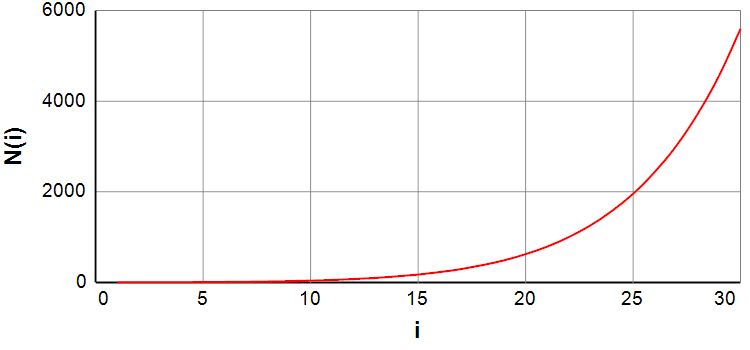
\includegraphics[scale=0.5]{Export/Complexity1.png}
\end{center}

Detta gör att man ställer sig frågan om denna talföljd är asymptotisk och växer på ett förutbestämt sätt, liknande andra välkända rekursivt definierade talföljder, exempelvis \emph{Fibonacci}-följden. Vi börjar därför med att definiera en rekursiv formel för beräkningen av antalet multiplicitetsföljder $N_i$ vars multipliciteter summerar till $i$:

\[
\begin{array}{rcl}
N_i & \equiv & N_{i,i} \\[5pt]
N_{i,j} & = & \left\{
\begin{array}{ll}
0 & , i < 0 \vee j \leq 0\\[5pt]
1 & ,i=0 \wedge j > 0\\[5pt]
\displaystyle\sum_{k=1}^{\min(i,j)}N_{i-k,k} & ,i>0 \wedge j>0\\
\end{array}
\right.\\
\end{array}
\]

Om $i>0$ motsvarar heltalet $i$ summan av multipliciteterna i de multiplicitetsföljder som $N_{i,j}$ beräknar. Vi sätter $N_{0,j} \equiv 1$ för att summeringen ska räkna varje följd en gång. Heltalet $j$ motsvarar den största tillåtna multipliciteten i följderna. Som vi kan se är rekursionen som definierar vår talföljd inte riktigt lika enkel då den är definierad i två dimensioner, samt innehåller en summa med en växande mängd termer. Den innehåller också en begränsning i det att en multiplicitet alltid begränsar storleken på efterföljande multipliciteter, vilket kan begränsa tillväxten av $N_i$.

För att uppskatta komplexiteten hos $N_i$ och hur den växer med $i$, ska vi i detta avsnitt empiriskt\footnote{For numeriska beräkningar har vi använt \emph{Clayster Script} \cite{ClaysterScript}, en skriptmotor för numeriska beräkningar utvecklad av Peter Waher.} studera kurvan för att se om vi kan hitta en enkel matematisk modell som passar den bra. Försöker vi med hjälp av minsta kvadratmetoden passa in polynom på denna kurva kommer vi inte hitta någon som passar. Istället ser vi hur termerna i polynomen alternerar mellan positiva och negativa, i takt med att vi försöker med högre och högre grader, något som kan indikera en exponentiell tillväxt, vilket vi misstänkt från början, även om det finns inbäddade beroenden som borde reducera komplexiteten något.

För att se om kurvan är exponentiell kan vi börja med att betrakta den naturliga logaritmen av antalet multiplicitetsföljder. Dock är den inte heller linjär. Istället visar den en svagt konkav kurva. För att se om det rör sig om en kvadratrot, ritar vi också ut kvadraten på logaritmen. Men denna är istället konvex. Ritar vi ut $\ln(N_i)^{3/2}$, får vi en kurva som i alla fall för ögat ser ut att vara mer eller mindre linjär:

\begin{center}
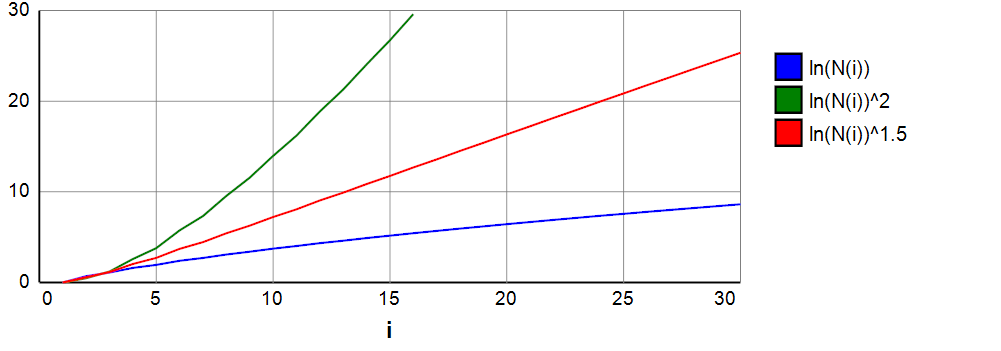
\includegraphics[scale=0.5]{Export/Complexity2.png}
\end{center}

Så, vi kan börja med ett empiriskt antagande, att $\ln(N_i)^E$ växer linjärt för någon exponent $E$:
\[\ln(N_i)^E \approx a+b\cdot i\]
\[\Longleftrightarrow\]
\[N_i \approx e^{(a+b\cdot i)^{\frac{1}{E}}} \]

För att avgöra vilken exponent som ger det bästa resultatet, kan vi enkelt beräkna kvadratfelet $\text{SE}(E)$ mellan $N_i$ och $e^{(a+b\cdot i)^{1/E}}$ och minimera den. I beräkningen av $\text{SE}(E)$ ser vi till att med linjär regression beräkna motsvarande $a$ och $b$ för varje exponent $E$ utifrån det data vi har. $\text{SE}'(E)$ uppvisar trevliga egenskaper och att hitta det bästa $E$ är lätt.

\[
\begin{array}{cc}
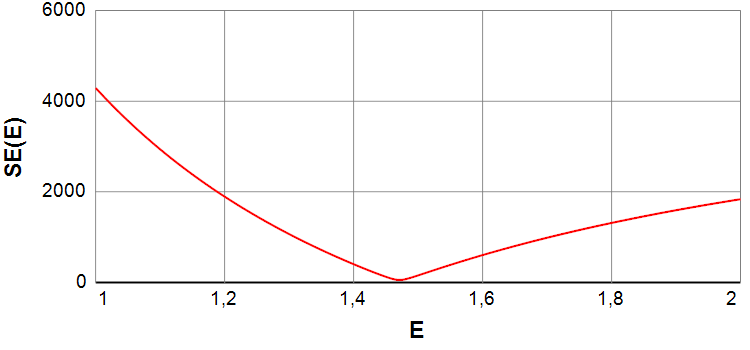
\includegraphics[scale=0.35]{Export/Complexity3.png}
&
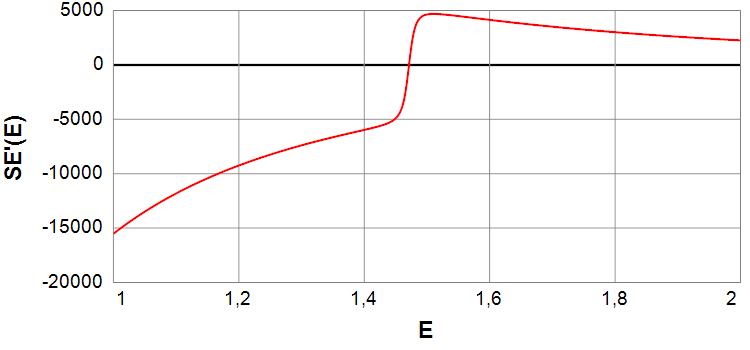
\includegraphics[scale=0.35]{Export/Complexity4.png}\\
\end{array}
\]
\[E=1.47126405685409, a=-1.34861467338489, b=0.839860447173521\]
Vi kan nu jämföra vår modell med det uppmätta värdena, för att se hur väl de stämmer överens. Till synes ganska väl, även om det inte är perfekt.
\[
\begin{array}{cc}
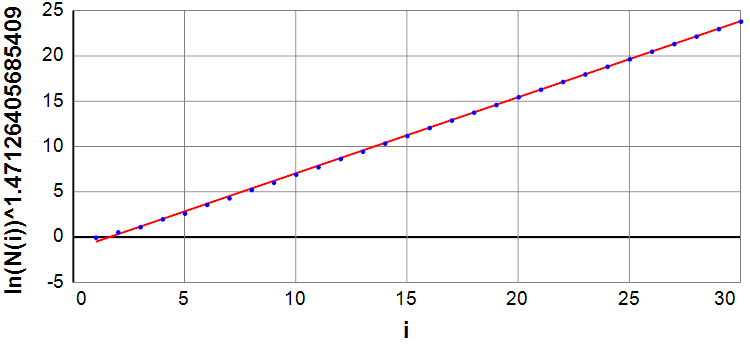
\includegraphics[scale=0.35]{Export/Complexity5.png}
&
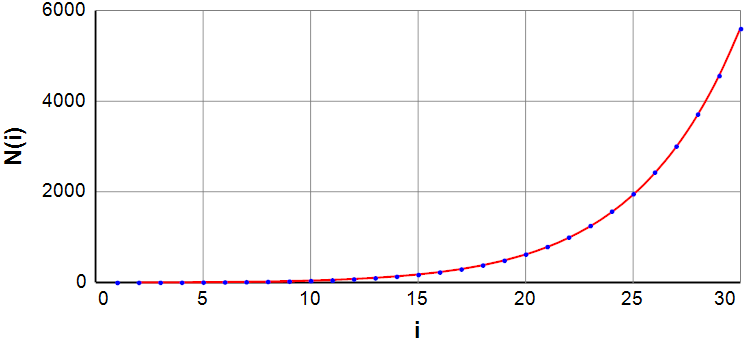
\includegraphics[scale=0.35]{Export/Complexity6.png}\\
\end{array}
\]

Visar vi istället skillnaden mellan uppmätt och uppskattat i fallet med $\ln(N_i)$ och felet mellan uppmätt och uppskattat i fallet med $N_i$ ser vi att vår uppskattning antagligen inte kommer att hålla när vi utökar våra beräkningar till ett större område, då felet ger en antydan till att kunna divergera då $i$ växer:
\[
\begin{array}{cc}
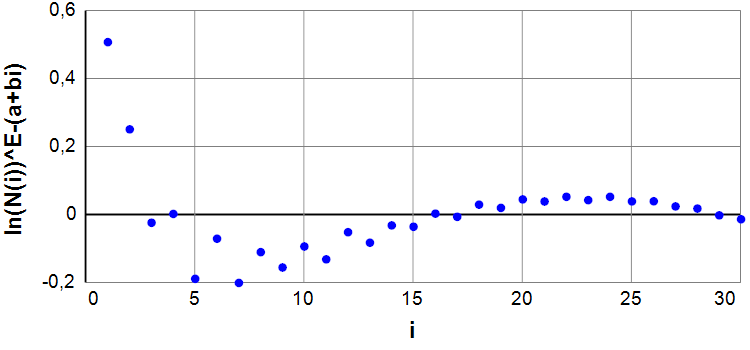
\includegraphics[scale=0.35]{Export/Complexity7.png}
&
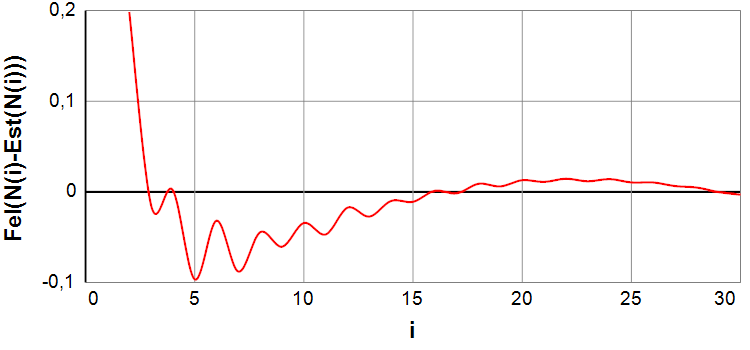
\includegraphics[scale=0.35]{Export/Complexity8.png}\\
\end{array}
\]

Men för att kunna beräkna fler $N_i$ kan vi inte använda oss av metoden i bilaga \ref{TestFindFunctionXYFromMultiplicitySequence}, där vi testar alla multiplicitetsföljder. Det är för tidskrävande. Istället implementerar vi en funktion som enbart beräknar rekursionsformeln för $N_i$. Med implementationen beskriven i bilaga \ref{FindNrMultiplicitySequences} på sidan \pageref{FindNrMultiplicitySequences} kan vi beräkna $N_i$ ända upp till $i=100$, under loppet av några timmar. Tyvärr visar dessa nya värden, att vår modell inte är riktigt korrekt. Det som är den bästa linjen på intervallet $[1,30]$ är inte den bästa linjen på intervallet $[1,100]$. En liten skillnad i exponenten ger ett stort absolut fel.

\[
\begin{array}{cc}
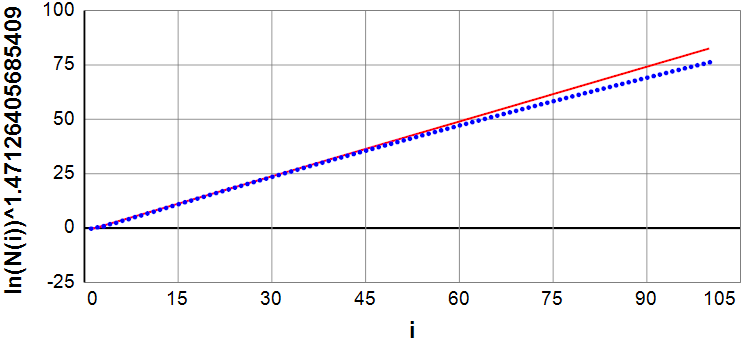
\includegraphics[scale=0.35]{Export/Complexity9.png}
&
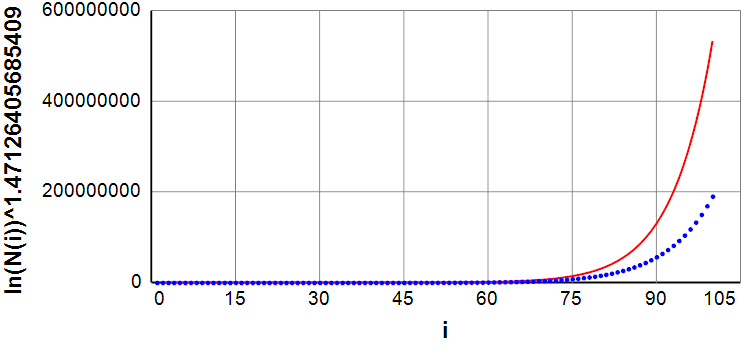
\includegraphics[scale=0.35]{Export/Complexity10.png}\\
\end{array}
\]

Som det ser ut verkar exponenten avta med stigande $i$. Vår exponentiella modell verkar inte helt korrekt, även om det kanske är en bra första ansats. Frågan är då, kommer den gå asymptotiskt mot en geometrisk serie $N_i \rightarrow c\cdot P^i$? Eller kommer $N_{i+1}/N_i \rightarrow 1$ då $i \rightarrow \infty$. dvs. begränsningarna i den rekursiva deklarationen kommer till slut göra så att $N_i$ långsamt slutar växa exponentiellt. Vi kan formulera om detta, genom att jämföra $N_i$ med en geometrisk talföljd: Om $Q_i=N_i/N_{i-1}$, kommer då $Q_i \rightarrow P$ för något $P$? Dvs. kommer $N_i \rightarrow c\cdot P^i$ då $i \rightarrow \infty$? Eller kommer den avta asymptotiskt mot 1? Om vi visualiserar $Q_i$ ser vi hur den avtar.

\begin{center}
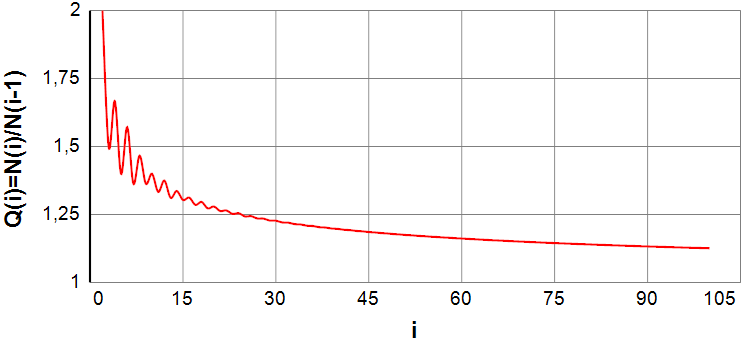
\includegraphics[scale=0.5]{Export/Complexity11.png}
\end{center}

För att få en bättre idé angående svaret på dena fråga, behöver vi beräkna $N_i$ för mycket högre värden på $i$. Maple-metoden i bilaga \ref{FindNrMultiplicitySequences} duger inte den heller. Maple är för långsamt för denna typ av beräkningar. Istället har vi tagit fram ett litet program i C\# \cite{GitHub} som utnyttjar en dators fulla kapacitet för att beräkna stora värden på $N_i$. Den utnyttjar datorns samtliga processorkärnor för att utföra parallella beräkningar och en stor intern minnescache för att mellanlagra uträknade $N_{i,j}$ så de kan återvändas i följande beräkningar. Genom att utnyttja detta har vi lyckats beräkna $N_i$ upp till $i=10000$. Dessutom beräknar programmet motsvarande serie ${Q_i}$. Vad vi får är:

\begin{center}
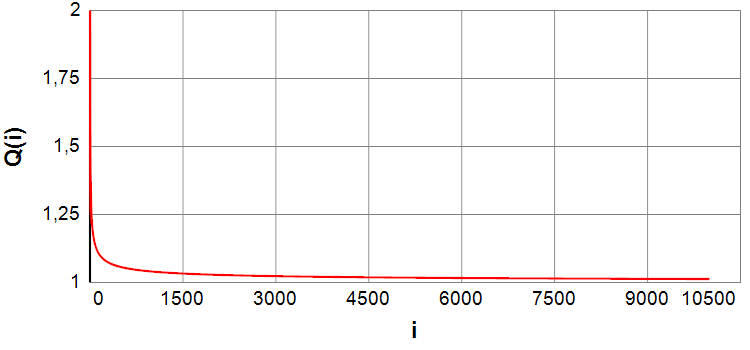
\includegraphics[scale=0.5]{Export/Complexity12.png}
\end{center}
\[
\begin{array}{rcl}
N_{10000} & = & 361672513256362939888204718909536954950160303393156\ldots\\
& & \ldots504220818686058879525687540664205923105560529069\ldots\\
& & \ldots16435144\\
Q_{10000} & = & 1.0128073565554...
\end{array}
\]

Det ser onekligen ut som om följden $Q_i=N_i/N_{i-1}$ avtar asymptotiskt mot 1, och inte mot ett tal $P>1$. Detta skulle således betyda att tillväxten inte är exponentiell. För att se om $Q_i$ motsvarar en invers, tittar vi på $1/(Q_i-1)$. Vi ser att kurvan är konkav och tittar således även på potenserna $1/(Q_i-1)^2$ och $1/(Q_i-1)^3$. Vi ser genast något väldigt intressant. $1/(Q_i-1)^2$ verkar vara en helt rät linje.

\begin{center}
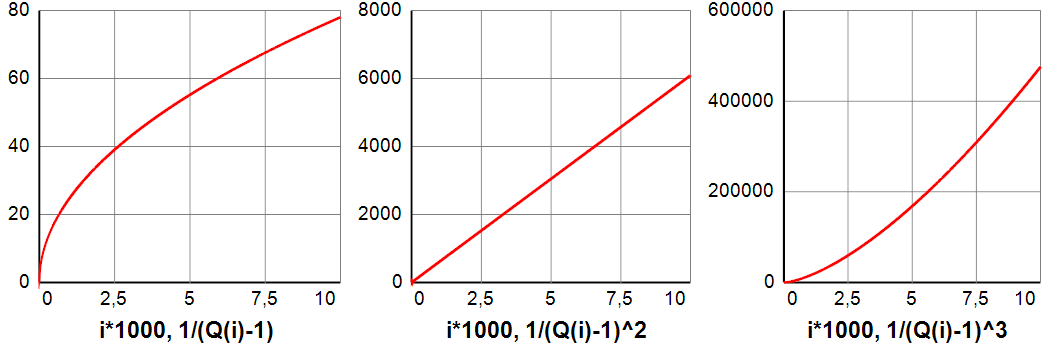
\includegraphics[scale=0.5]{Export/Complexity13.png}
\end{center}

För att försäkra oss om vilken exponent som ger den mest räta linjen, skapar vi en funktion $\text{SEQ}(E)$ som beräknar det kvadratiska felet mellan den bästa linjen och det uträknade datat, givet en exponent $E$. Den resulterande kurvan och dess derivata $\text{SEQ}'(E)$ uppvisar en väldigt tydlig lösning inom det intervall vi studerat.

\[
\begin{array}{cc}
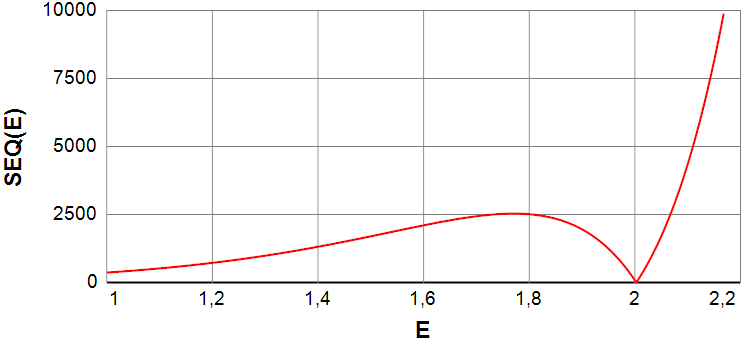
\includegraphics[scale=0.35]{Export/Complexity14.png}
&
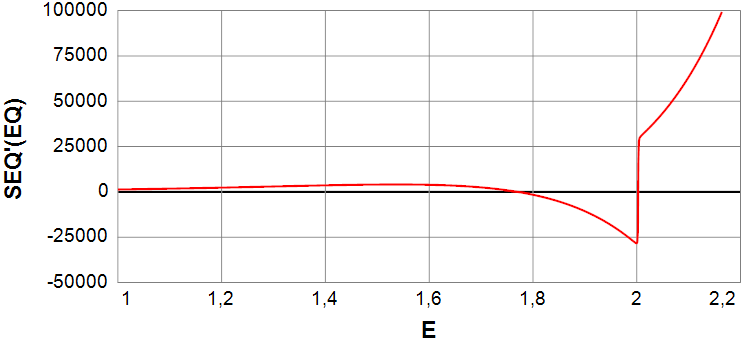
\includegraphics[scale=0.35]{Export/Complexity15.png}\\
\end{array}
\]
\[E_{[1,10000]} = 2.00264350576171\]

För att se hur denna lösning beror på det intervall vi studerat ($Q_1-Q_{10000}$), gör vi samma beräkning för olika intervall på området. I grafen nedan finns två kurvor. För den röda (den översta) används alla data upp till ett givet $Q_{max}$. För den blåa (den undre) används alla data från ett givet $Q_{min}$. Som vi ser varierar inte exponenten nämnvärt som den gjorde då vi undersökte en exponentiell modell. Dessutom är den undre ``bättre'', om vi förväntar oss att kurvorna asymptotiskt går mot 2, vilket de ser ut att kunna göra båda två.

\begin{center}
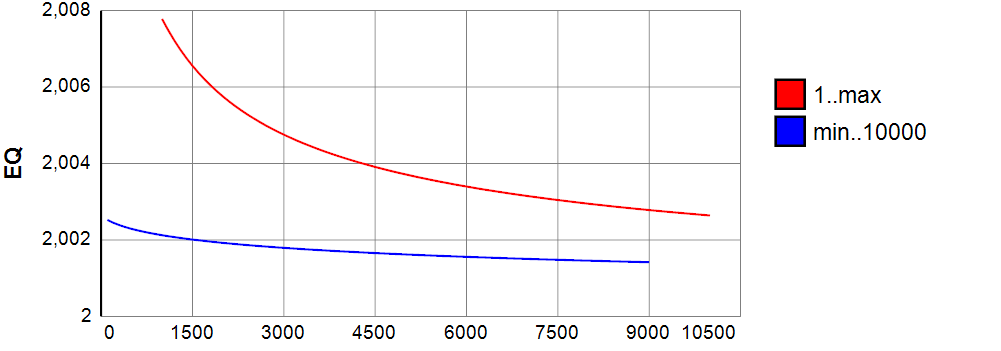
\includegraphics[scale=0.5]{Export/Complexity16.png}
\end{center}
\[E_{[9000,10000]} = 2.00142039633785\]

Från vår empiriska studie över antalet multiplicitetsföljder $N_i$, och dess förhållanden $Q_i=N_i/N_{i-1}$, är det således inte helt orimligt att göra följande antagande angående $Q_i$'s asymptotiska beteende:

\[\frac{1}{\left(Q_i-1\right)^2} \sim a+b\cdot i \text{, (då $i \rightarrow \infty$)}\]
\[\Longleftrightarrow \]
\[Q_i \sim 1+\frac{1}{\sqrt{a+b\cdot i}} \]

För att hitta koefficienterna skapar vi en modellfunktion $f_\mathbf{v}(i)$, med en parametervektor $\mathbf{v}$ som vi sedan med hjälp av \emph{Nelder-Mead's algoritm} \cite{NelderMead} optimerar så att felet mellan $f_\mathbf{v}(i)$ och $Q_i$ blir så litet som möjligt. Vi lägger på lite fler potenser för att se hur dessa påverkar. Vi definierar $f_\mathbf{v}(i)$ så här:
\[f_\mathbf{v}(i)=v_0+\frac{v_1}{\sqrt{v_2+v_3\cdot i+v_4\cdot i^2+v_5\cdot i^3+v_6\cdot i^4+v_7\cdot i^5+v_8\cdot i^6+v_9\cdot i^7}}\]

\emph{Nelder-Mead's algoritm} garanterar inte ett globalt minimum i felfunktionen, utan hittar bara ett lokalt sådant. Resultatet beror på vår initiala gissning. Men vi har redan en relativt kvalificerad gissning ovan. De extra potenserna har vi lagt dit för att se om algoritmen föreslår att någon av dessa potenser bör ingå. Algoritmen använder sig inte av funktionens derivator\footnote{Försök gjordes med andra metoder, som sjunkgradientmetoden och Newtons metod i flera dimensioner, genom användning av numerisk uppskattning av gradient och Hessmatris, men dessa metoder var svåra att få att konvergera, även med hjälp av dämpningskoefficient.} för att söka efter bästa $\mathbf{v}$, utan använder istället en uppsättning simplex i parameterrummet och sökning utifrån dessa för att ringa in området där minimum finns. Algoritmen föreslår följande parameteruppsättning utifrån vår gissning:
\[\text{NM}(f_\mathbf{v},\left\{1,1,1,1,0,0,0,0,0,0\right\})= \left\{1, 1.27124055101012, 1, 1, 0; 0; 0; 0; 0; 0\right\}\]
Vi har således fått en uppskattning av $Q_i$:
\[Q_i \approx 1+\frac{1.27124055101012}{\sqrt{1+i}} \]
Vi kan rita ut $Q_i$ tillsammans med sin uppskattning, och ser att de verkar stämma överens ganska bra:

\begin{center}
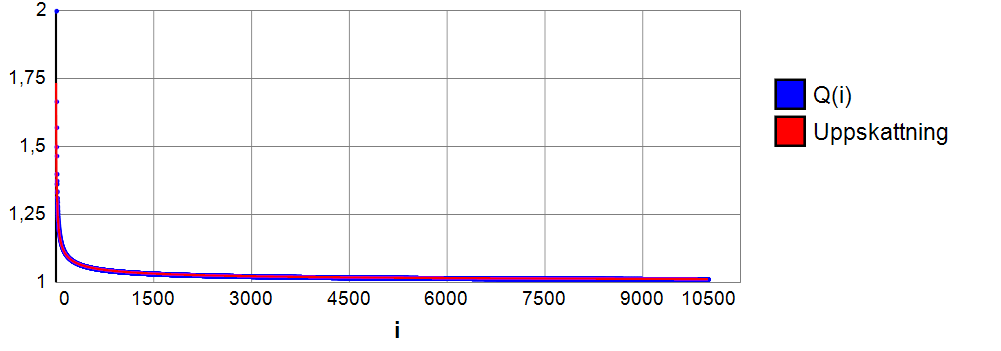
\includegraphics[scale=0.5]{Export/Complexity17.png}
\end{center}

Ännu bättre ser vi att de stämmer överens om vi ritar ut felet mellan $Q_i$ och dess uppskattning, $\text{Err}_Q(i)$:

\begin{center}
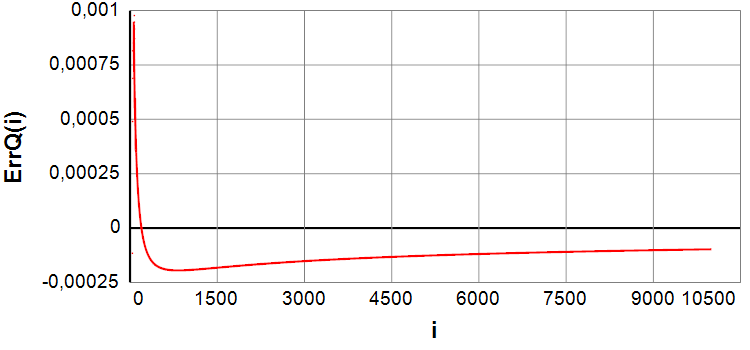
\includegraphics[scale=0.5]{Export/Complexity18.png}
\end{center}

Inte bara är felet litet, det verkar gå mot noll då $i$ växer, utan tendens att divergera. Vi kan således dra slutsatsen att $N_i$ \emph{inte} växer exponentiellt, i motsats till vad vi antog i början. Istället verkar den växa i enlighet med:
\[N_i = \prod_{k=1}^{i} Q_i = \prod_{k=1}^{i} \left(1+\frac{1.27124055101012}{\sqrt{1+k}}+\text{Err}_Q(k)\right) \]
där $\text{Err}_Q(k)$ verkar gå mot 0 då $k \rightarrow \infty$. Dock har felet i uppskattningen av $Q_i$ väldigt stor påverkan på den multiplikativa uppskattningen av $N_i$, som kan ses av följande graf som är förhållandet mellan $N_i$ och
\[N^-_i=\prod_{k=1}^{i} \left(1+\frac{1.27124055101012}{\sqrt{1+k}}\right)\]

\begin{center}
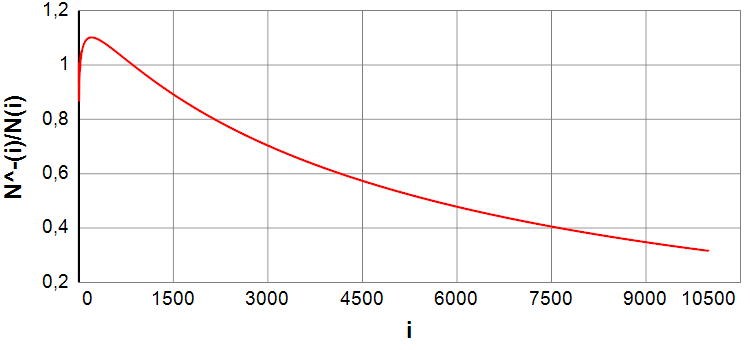
\includegraphics[scale=0.5]{Export/Complexity19.png}
\end{center}

Vi ser att efter $i=856$ gäller att $N_i>N^-_i$. Vi vet också att $\text{Err}_Q(856) \approx -0.000194294156604657$, och att $\text{Err}_Q(i)$ är svagt växande därefter. Vi kan därför skapa en övre gräns för $N_i$, då $i \geq 856$ på följande sätt:
\[N^+_i = N_{856} \cdot \prod_{k=1}^{i} \left(1+\frac{1.27124055101012}{\sqrt{1+k}}-\text{Err}_Q(856)\right), i\geq 856 \]

Vi får då en begränsning av $N_i$ enligt $N^-_i \leq N_i \leq N^+(i), i\geq 856$, vilket illustreras som följer.

\begin{center}
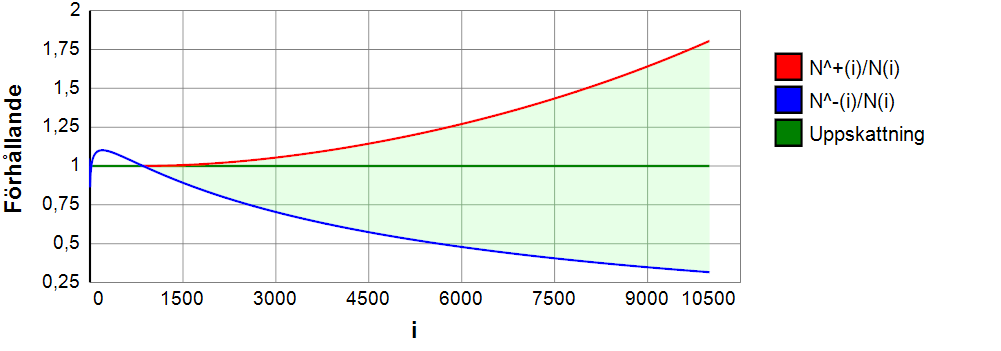
\includegraphics[scale=0.5]{Export/Complexity20.png}
\end{center}

Vi har med empiriska metoder kunnat påvisa att $N_i$ inte växer exponentiellt, utan bäst verkar beskrivas som en serie produkter med avtagande faktorer, där vi påvisat en tydlig trend hos $Q_i$ och hur dessa verkar avta asymptotiskt mot 1, samt i vilken takt. Vi har också gjort en uppskattning som begränsar $N_i$ på ett tydligt sätt, för att få en uppfattning av komplexiteten hos algoritmer som baseras på mängden multiplicitetsföljder. Inom ramen för detta arbete presenteras inget faktiskt bevis för att dessa empiriska resultat stämmer. Detta överlåts på framtiden åt hågade specialister inom kombinatorik.